%========================================================================
% Modelo para elaboracao de textos academicos: TCC, dissertacoes e teses
% Elaborado pelo GISIS - Grupo de Imageamento Sismico e Inversao Sismica.
%========================================================================
\chapter{Resultados}
\label{ch:resultados}

Neste capítulo, é apresentado os resultados da comparação entre os métodos de \citeonline{podvin1991finite}, \citeonline{jeong2008fast} e \citeonline{noble2014accurate} em termos de precisão no cálculo dos tempos de trânsito, desempenho computacional e recuperação dos modelos por inversão tomográfica. 

\subsection*{Comparação numérica}

Como parte de um experimento apresentado ao Simpósio Brasileiro de Geofísica em 2022, uma comparação numérica entre os métodos estudados será abordada, agora demonstrando valores de eficiência computacional, precisão e comportamento utilizando reciprocidade. O exemplo esquemático aloca uma fonte na superfície do modelo de velocidade e um arranjo circular de receptores espaçados regularmente de 50 metros com distância de 10 km da fonte. O modelo de velocidades empregado contém somente uma interface com propriedades de 1500 e 2000 m/s para cada camada. A figura \ref{fig:configurationNumericalComparison} mostra a configuração do experimento, o modelo de velocidades detalhado em forma de perfil e cortes do modelo com as isócronas de tempo projetadas. Para verificar a precisão dos métodos, foi construído três modelos de velocidade com espaçamentos de 25, 50 e 100 metros.  




\begin{figure}[H]
	\centering
	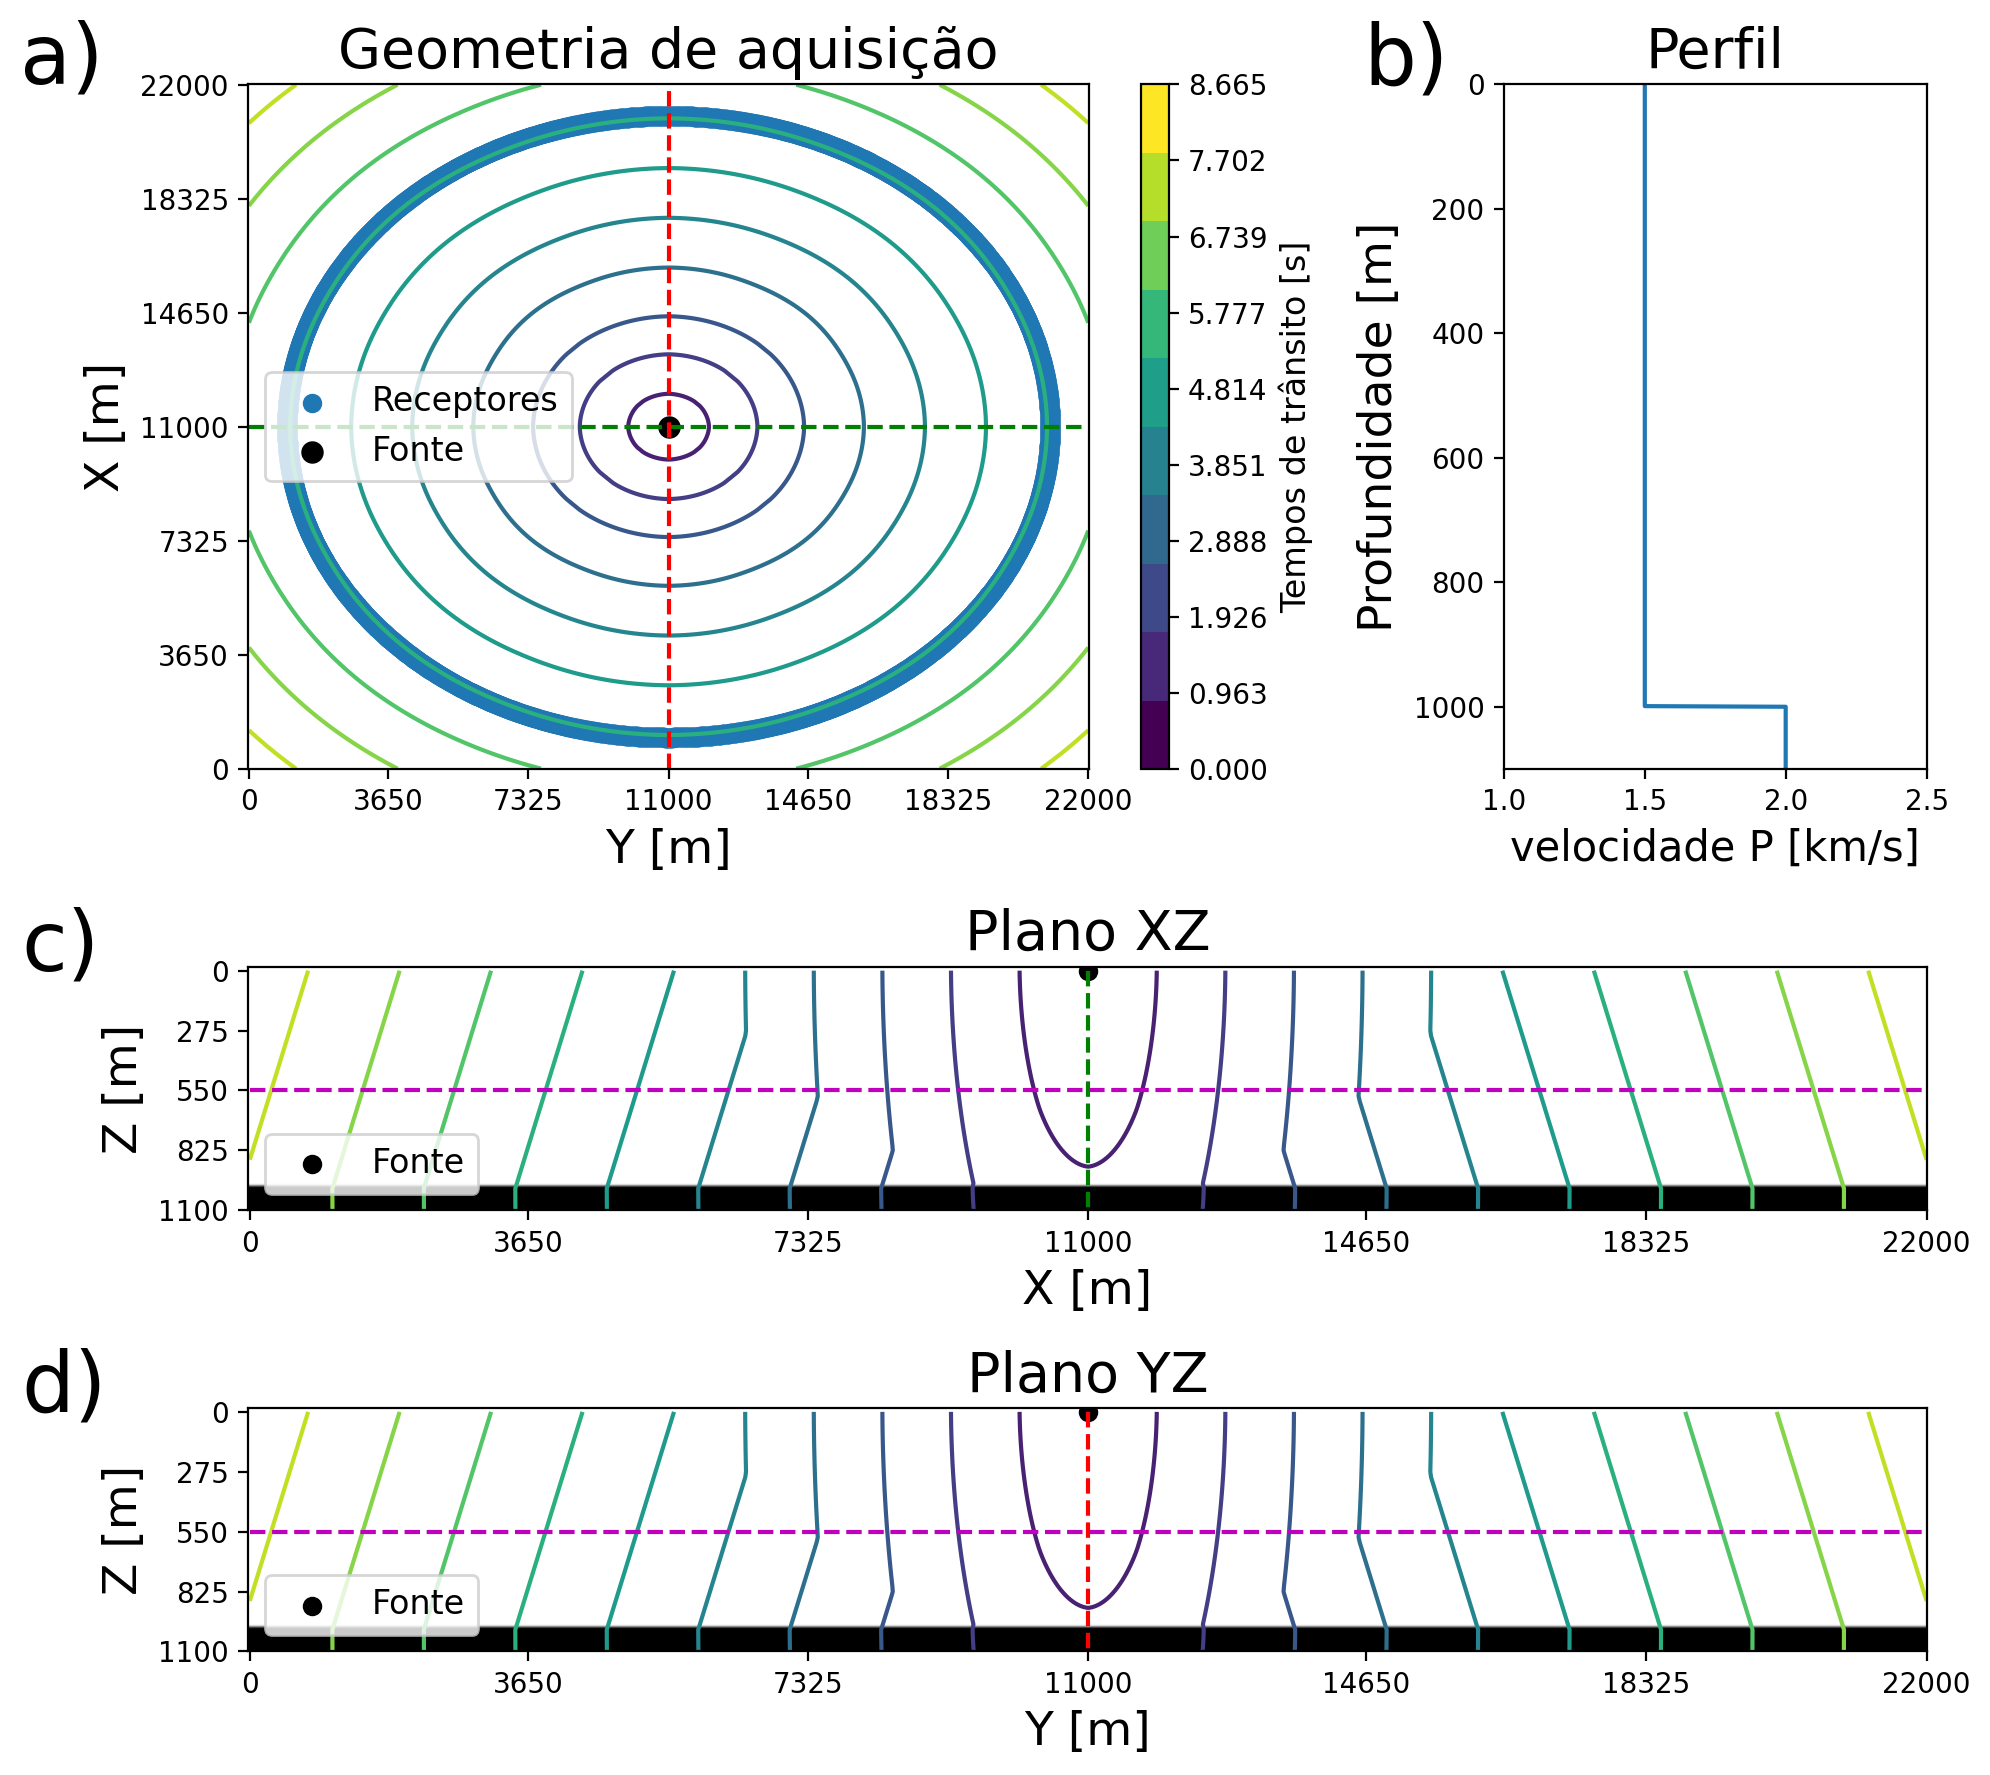
\includegraphics[width = 11cm, height = 10cm]{Imgs/RevisaoBibliografica/modelGeometry.png}
	\caption{Modelo empregado no teste de precisão e performance. (a) Plano XY ilustrando a geometria de aquisição com o arranjo de receptores circulares possuindo somente um tiro central. Isócronas mapeando o comportamento dos tempos de trânsito são mostradas. (b) Perfil de velocidades delimitando a posição da interface. (c) e (d) são as projeções dos cortes em planos XZ e YZ em relação à posição da fonte.}
	\label{fig:configurationNumericalComparison}
\end{figure}


\begin{figure}[H]
	\centering
	\subfloat[]{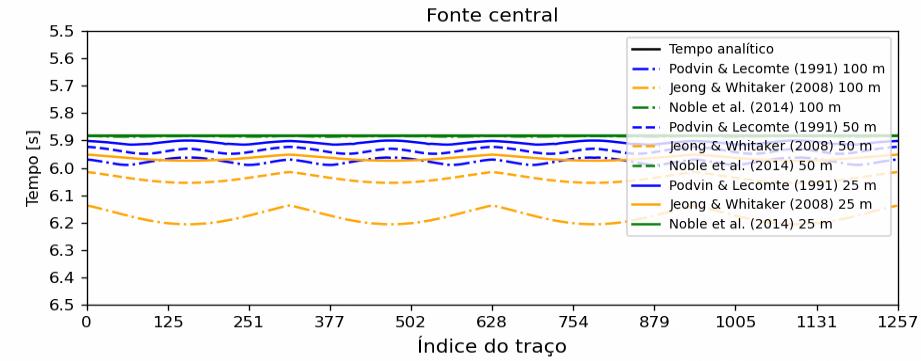
\includegraphics[width=8cm,height=3.5cm]{Imgs/RevisaoBibliografica/precision_direct.png}\label{fig:rnca}}
	\subfloat[]{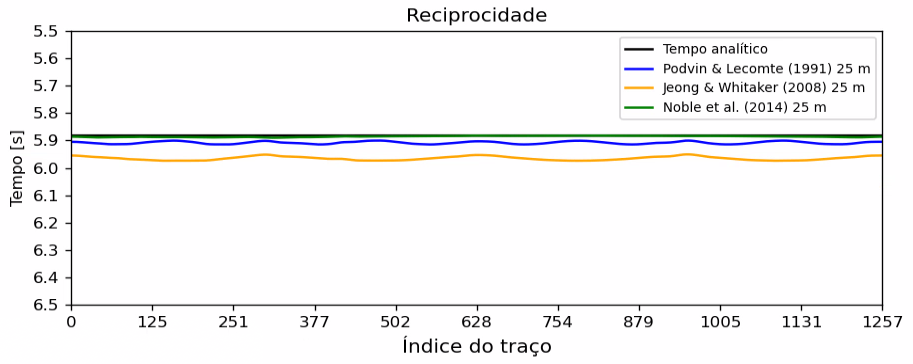
\includegraphics[width=8cm,height=3.5cm]{Imgs/RevisaoBibliografica/reciprocity.png}\label{fig:rncb}}
	
	\subfloat[]{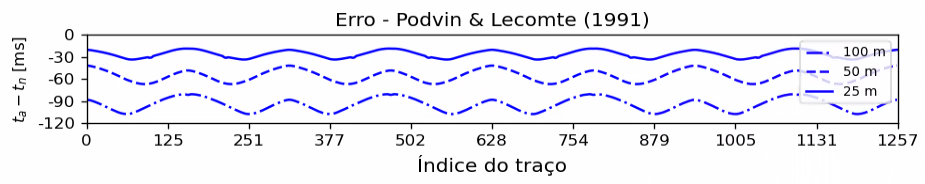
\includegraphics[width=8cm,height=1.5cm]{Imgs/RevisaoBibliografica/error_pod_direct.png}\label{fig:rncc}}
	\subfloat[]{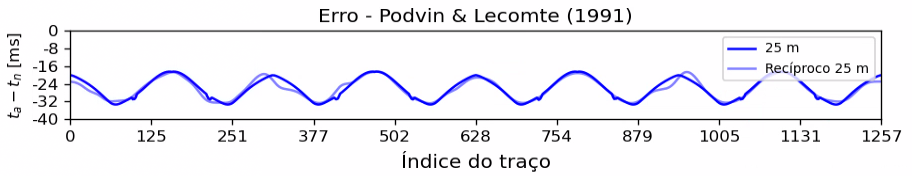
\includegraphics[width=8cm,height=1.5cm]{Imgs/RevisaoBibliografica/error_pod_reciprocity.png}\label{fig:rncd}}
	
	\subfloat[]{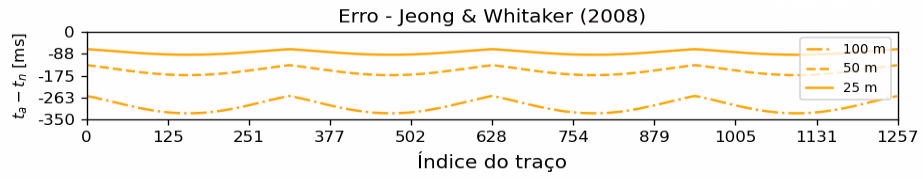
\includegraphics[width=8cm,height=1.5cm]{Imgs/RevisaoBibliografica/error_fim_direct.png}\label{fig:rnce}}
	\subfloat[]{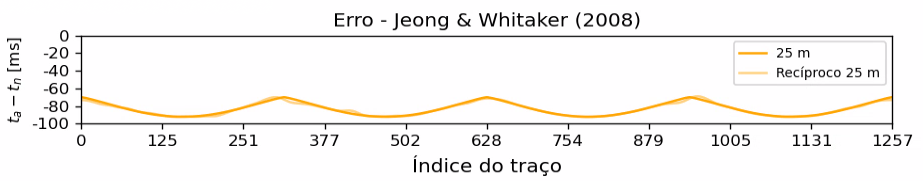
\includegraphics[width=8cm,height=1.5cm]{Imgs/RevisaoBibliografica/error_fim_reciprocity.png}\label{fig:rncf}}
	
	\subfloat[]{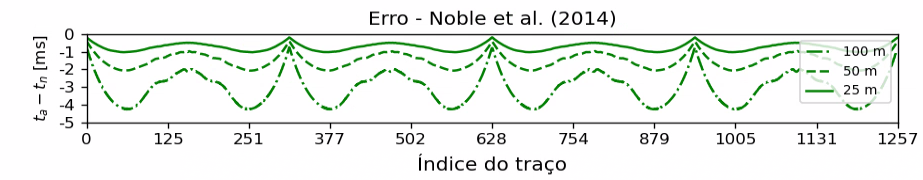
\includegraphics[width=8cm,height=1.5cm]{Imgs/RevisaoBibliografica/error_fsm_direct.png}\label{fig:rncg}}
	\subfloat[]{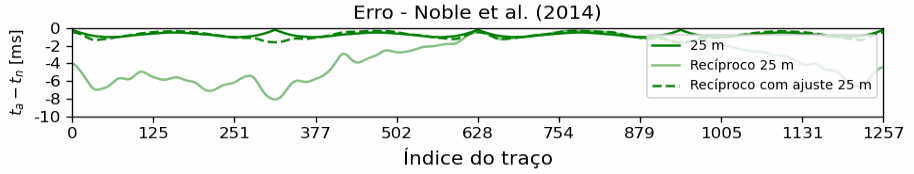
\includegraphics[width=8cm,height=1.5cm]{Imgs/RevisaoBibliografica/error_fsm_reciprocity.png}\label{fig:rnch}}
	
	\caption{Comparação de precisão entre os métodos numéricos estudados. (a) Mapeamento de todas as chegadas para os métodos numéricos testados para os espaçamentos estudados. (b) Estudo de reciprocidade utilizando o espaçamento de 25 m. (c) Escala do erro para as chegadas em diferentes espaçamentos e (d) tempo direto e recíproco utilizando a formulação de \citeonline{podvin1991finite}. (e) Escala do erro e (f) estudo de reciprocidade para a formulação de \citeonline{jeong2008fast}. (g) Escala do erro e (h) estudo de reciprocidade para a formulação de \citeonline{noble2014accurate}.}
	\label{fig:resultsNumericalComparison}
\end{figure}

\begin{table}[H]
	\begin{tabular}{|c|c|c|c|}
		\hline  
		Tipo                 & Método clássico & FIM       & FSM       \\ \hline
		100 m                & 0,0676 s        & 0,0491 s  & 0,1042 s  \\
		50 m                 & 0,3141 s        & 0,0987 s  & 0,2286 s  \\
		25 m                 & 3.5324 s        & 0.6261 s  & 0.8284 s  \\
		Reciprocidade (25 m) & 7896.2 s        & 921.8 s   & 1382.5    \\ \hline
	\end{tabular}
\end{table}






\section{Convergência tomográfica}

\begin{figure}[H]
	\centering
	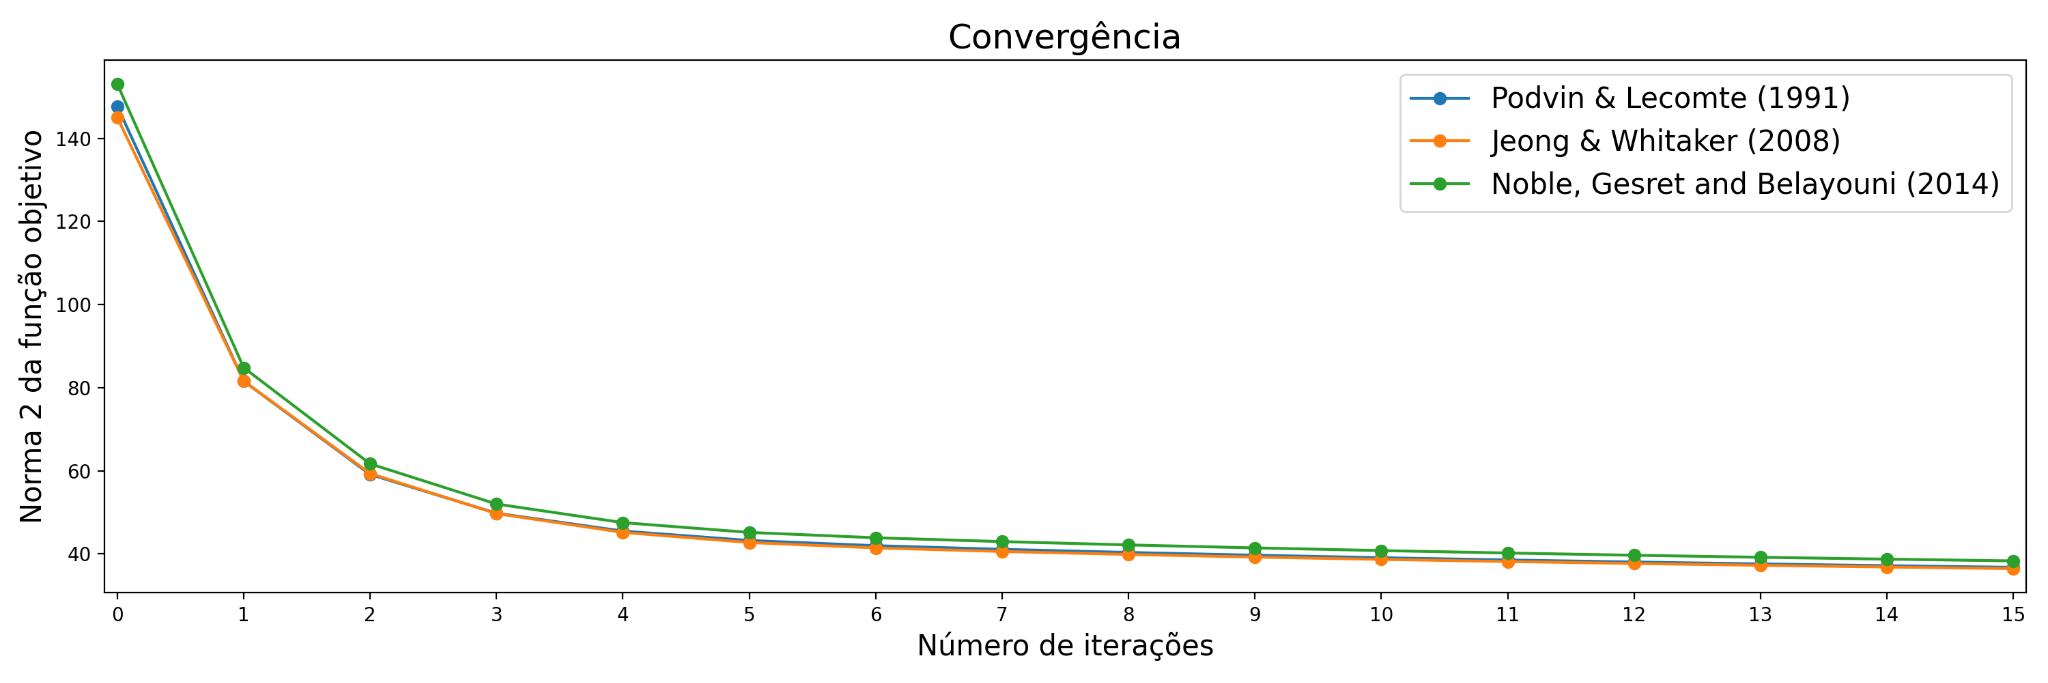
\includegraphics[width=16cm,height=6cm]{Imgs/Resultados/convergencia.png}
	\caption{Mapa de convergência tomográfica para os métodos estudados. Iterações entre 0 e 5 a malha esparsa foi aplicada no processo de inversão. Iterações entre 6 e 15 a malha refinada foi utilizada na tomografia.}
	\label{fig:convergencia}	
\end{figure}



\section{Inversão com malha esparsa}



\begin{figure}[H]
	\centering
	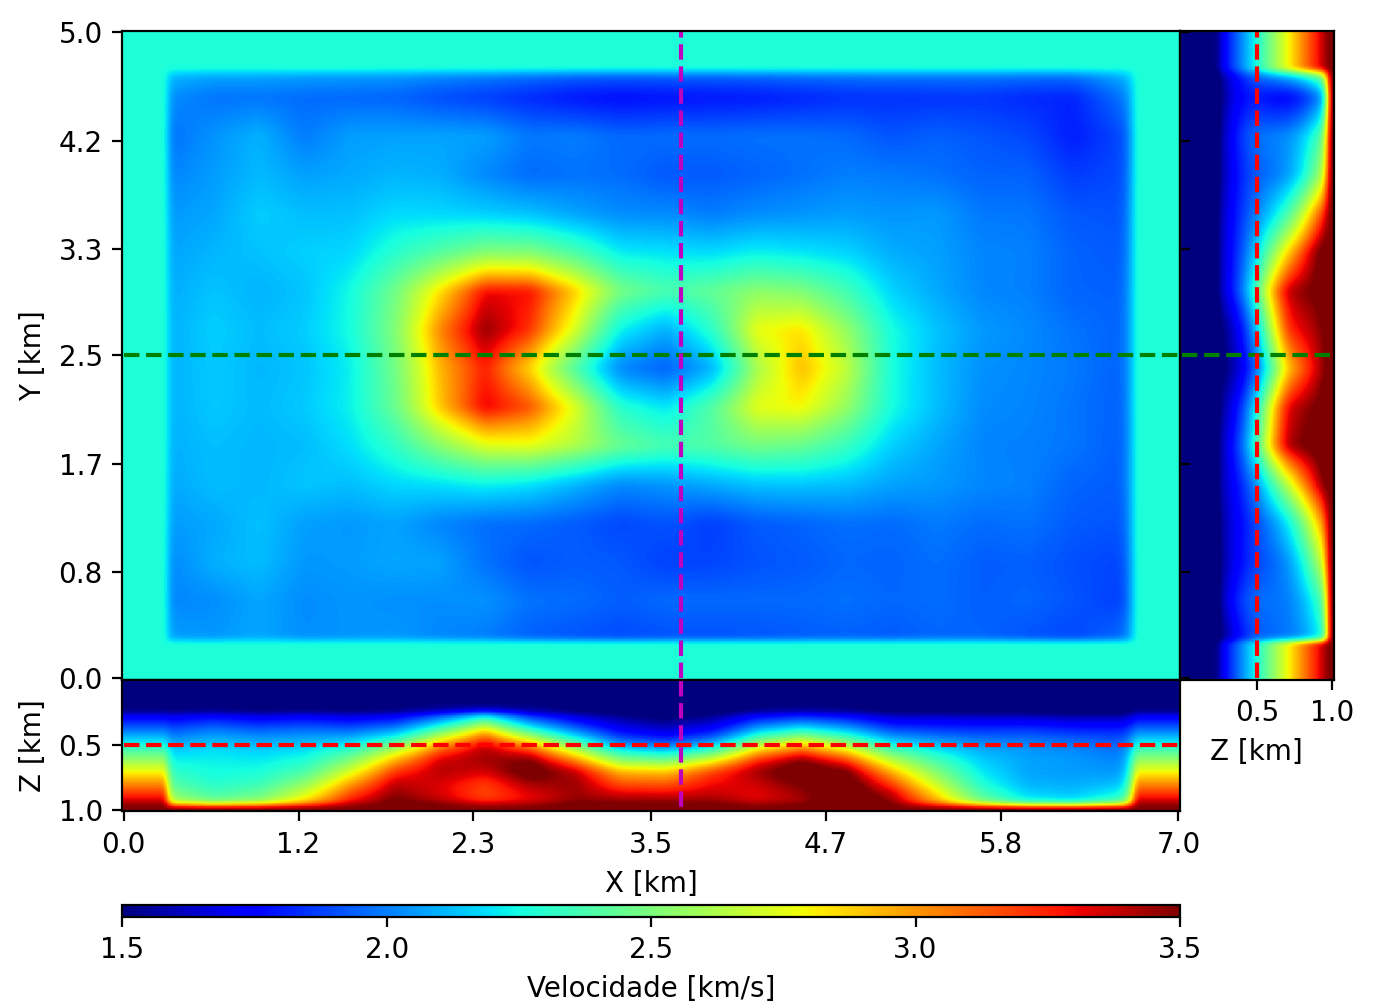
\includegraphics[width=12cm,height=9cm]{Imgs/Resultados/pod_sparse.png}
	\caption{Modelo recuperado utilizando a formulação de \citeonline{podvin1991finite}.}
	\label{fig:pod_sparse}	
\end{figure}


\begin{figure}[H]
	\centering
	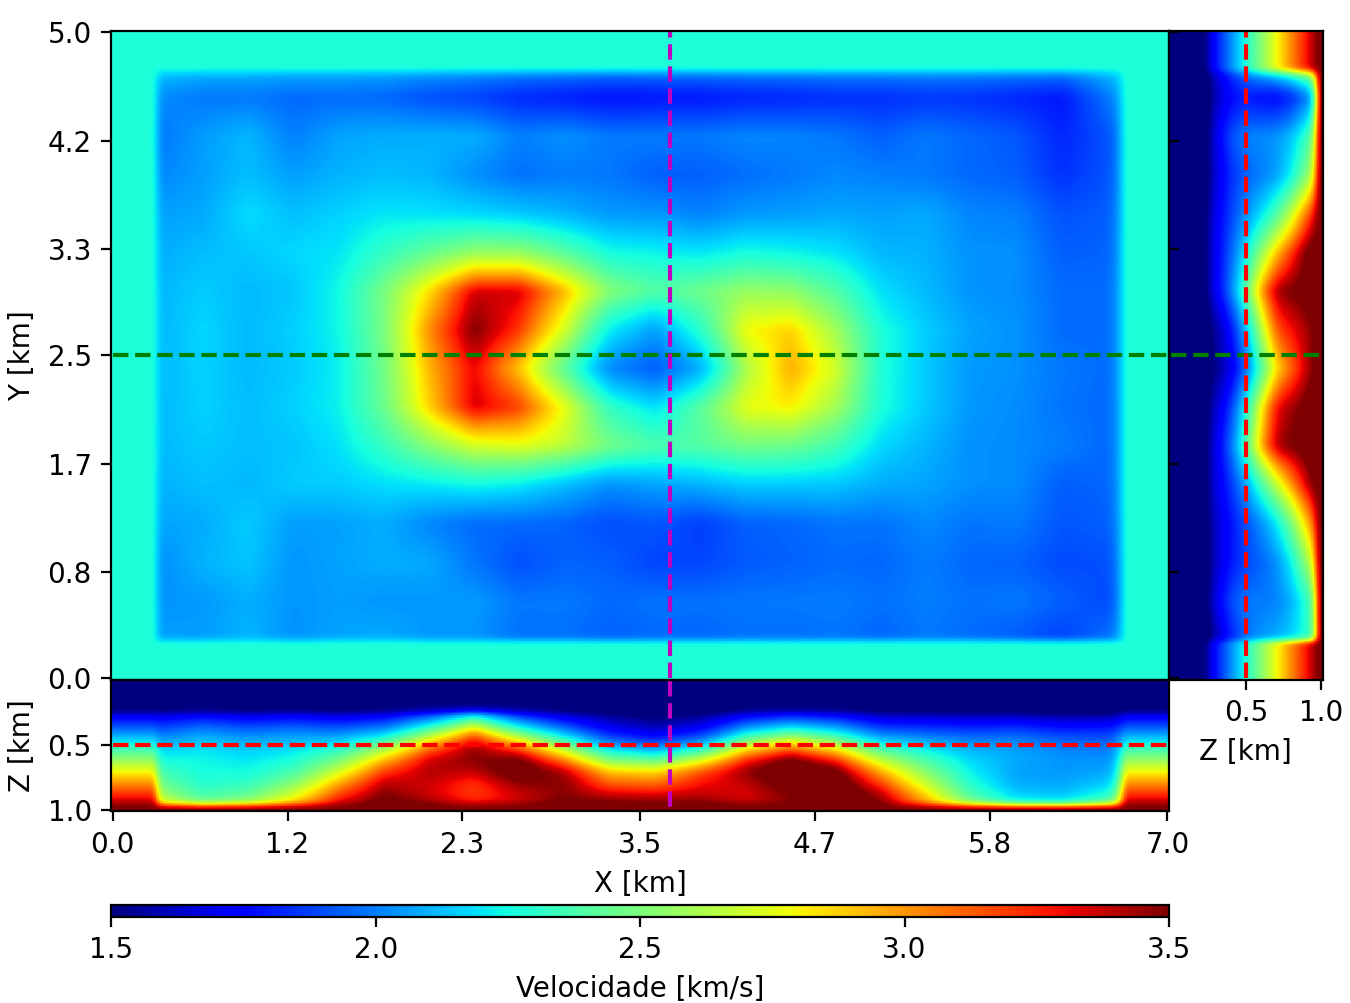
\includegraphics[width=12cm,height=9cm]{Imgs/Resultados/fim_sparse.png}
	\caption{Modelo recuperado utilizando a formulação de \citeonline{jeong2008fast}.}
	\label{fig:fim_sparse}	
\end{figure}


\begin{figure}[H]
	\centering
	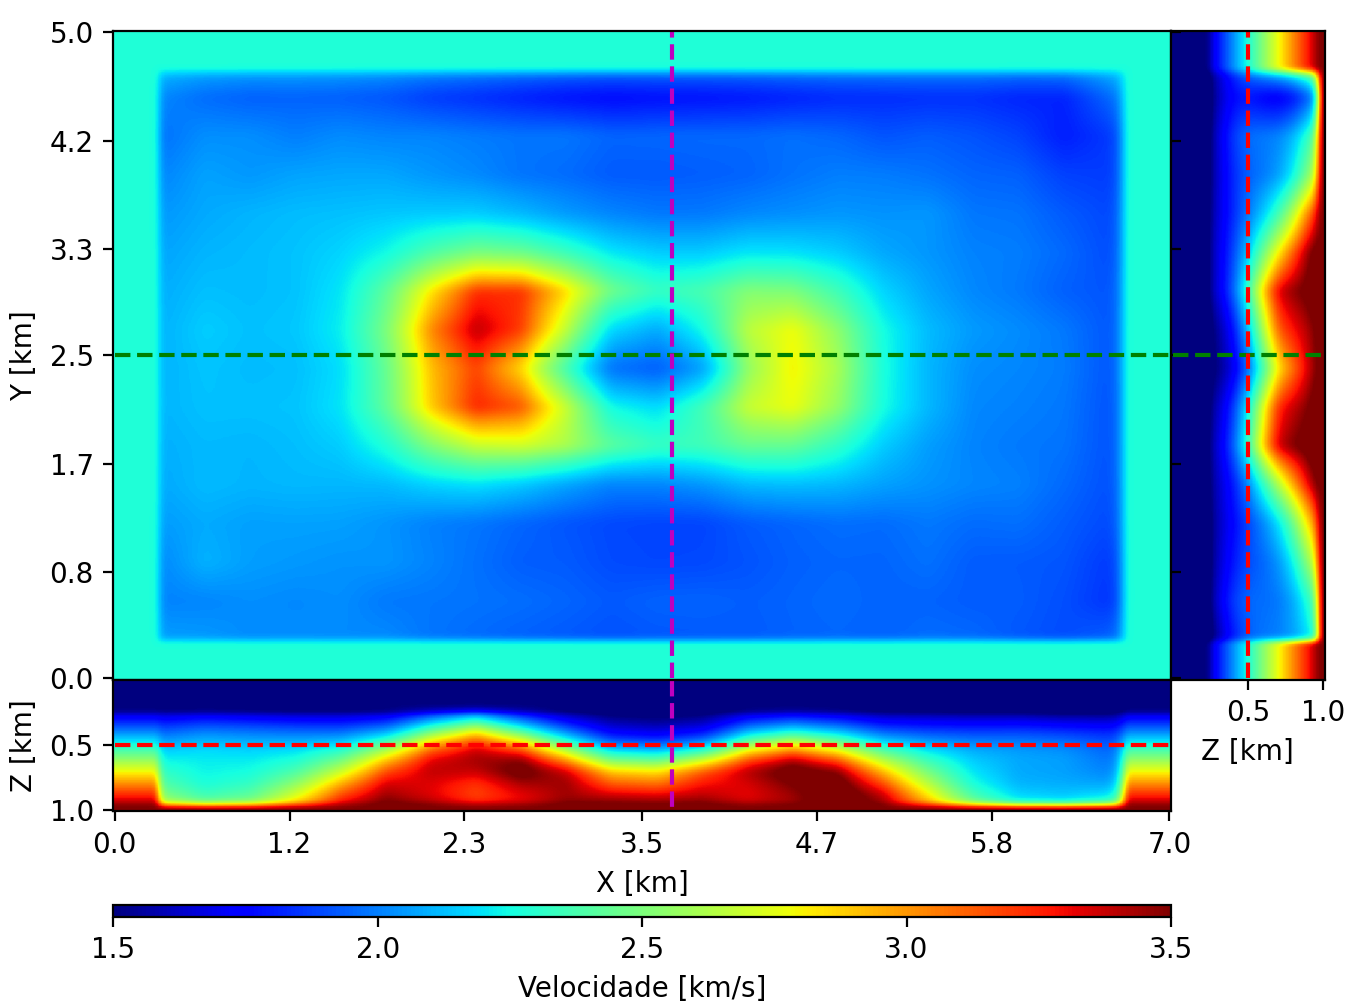
\includegraphics[width=12cm,height=9cm]{Imgs/Resultados/fsm_sparse.png}
	\caption{Modelo recuperado utilizando a formulação de \citeonline{noble2014accurate}.}
	\label{fig:fsm_sparse}	
\end{figure}


\section{Inversão com malha refinada}

\begin{figure}[H]
	\centering
	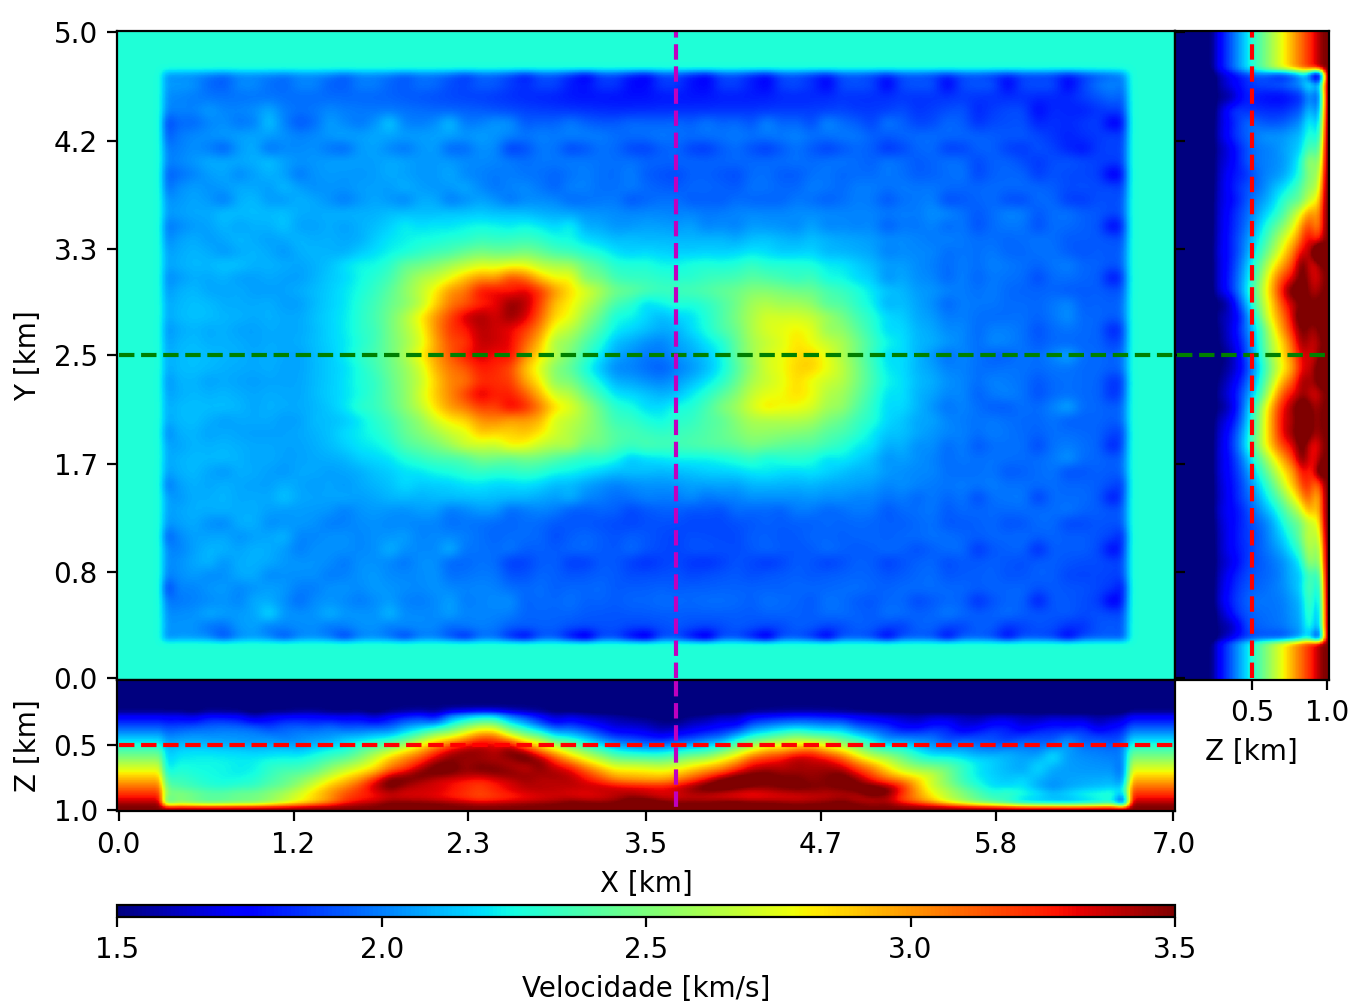
\includegraphics[width=12cm,height=9cm]{Imgs/Resultados/pod_refined.png}
	\caption{Modelo recuperado utilizando a formulação de \citeonline{podvin1991finite}.}
	\label{fig:pod_refined}	
\end{figure}


\begin{figure}[H]
	\centering
	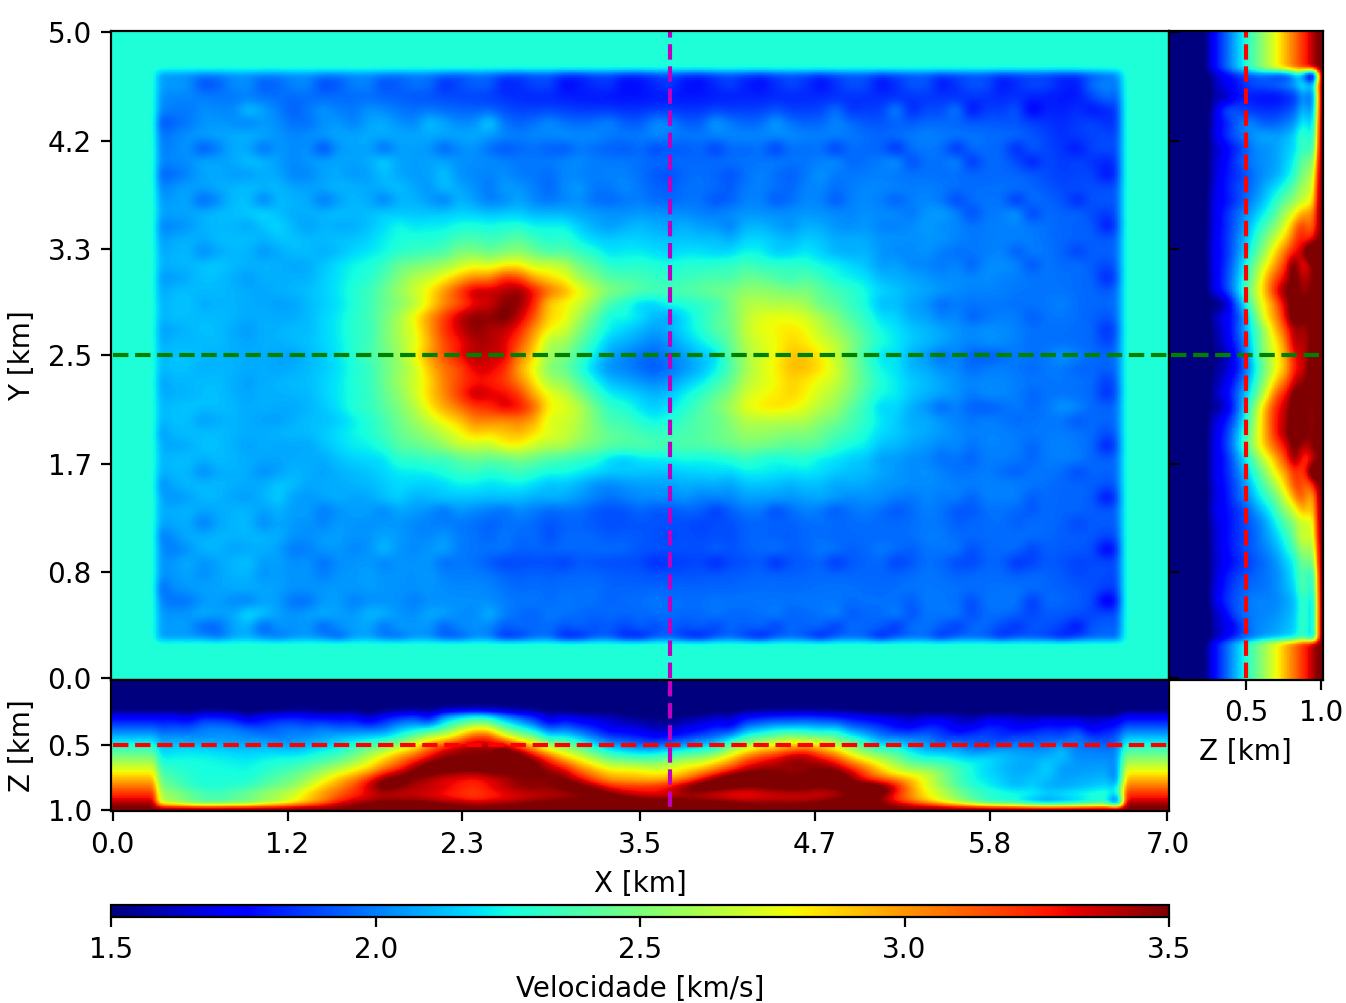
\includegraphics[width=12cm,height=9cm]{Imgs/Resultados/fim_refined.png}
	\caption{Modelo recuperado utilizando a formulação de \citeonline{jeong2008fast}.}
	\label{fig:fim_refined}	
\end{figure}


\begin{figure}[H]
	\centering
	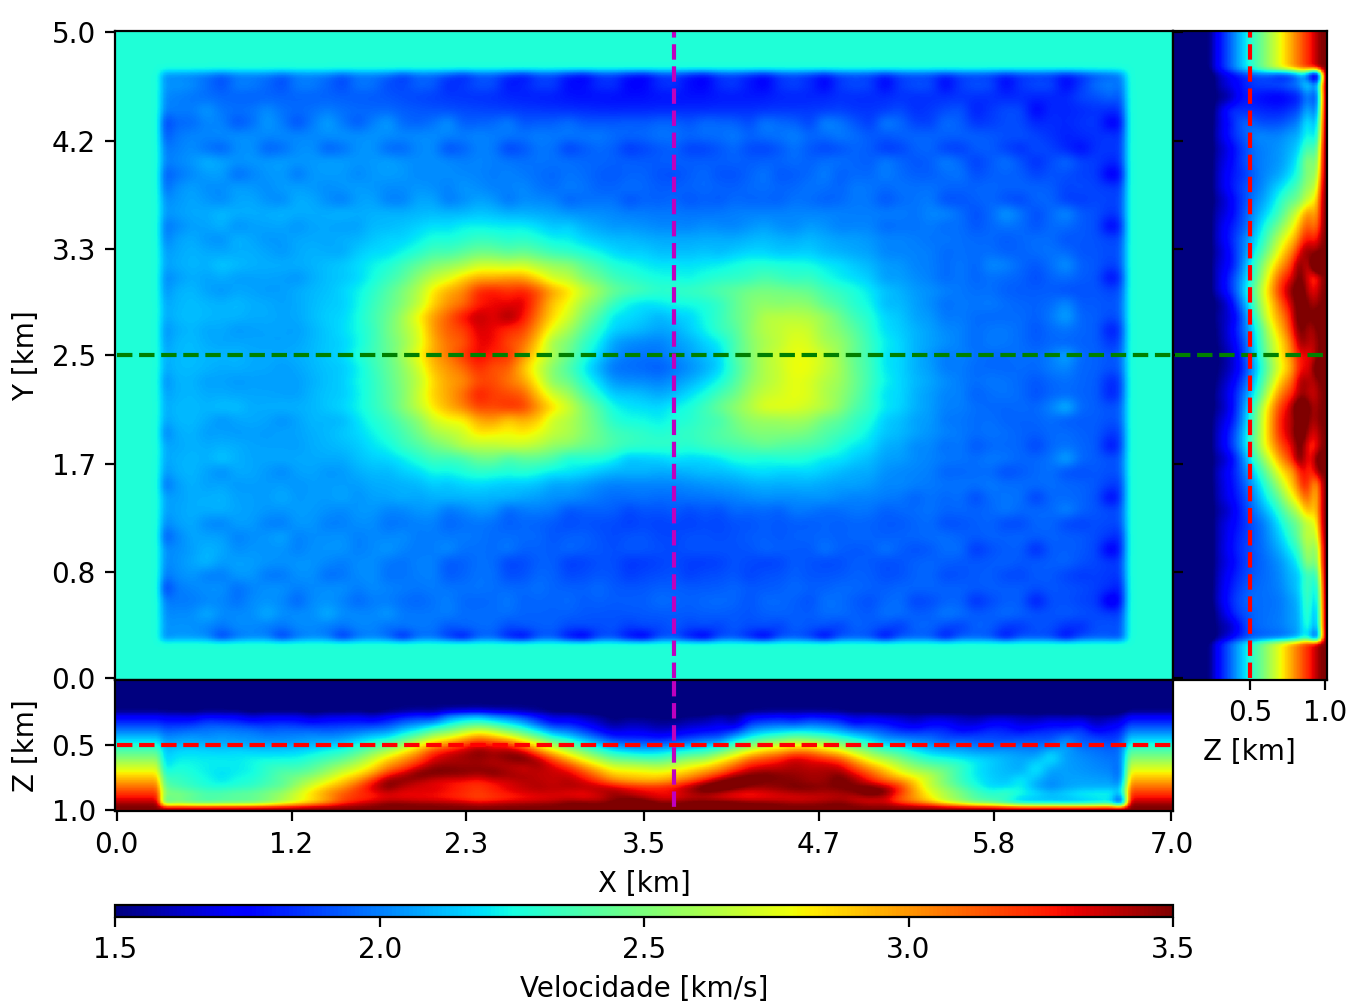
\includegraphics[width=12cm,height=9cm]{Imgs/Resultados/fsm_refined.png}
	\caption{Modelo recuperado utilizando a formulação de \citeonline{noble2014accurate}.}
	\label{fig:fsm_refined}	
\end{figure}





